\chapter{Einleitung}

\begin{figure}[H]
	\centering
	\begin{minipage}{.5\textwidth}
		\centering
		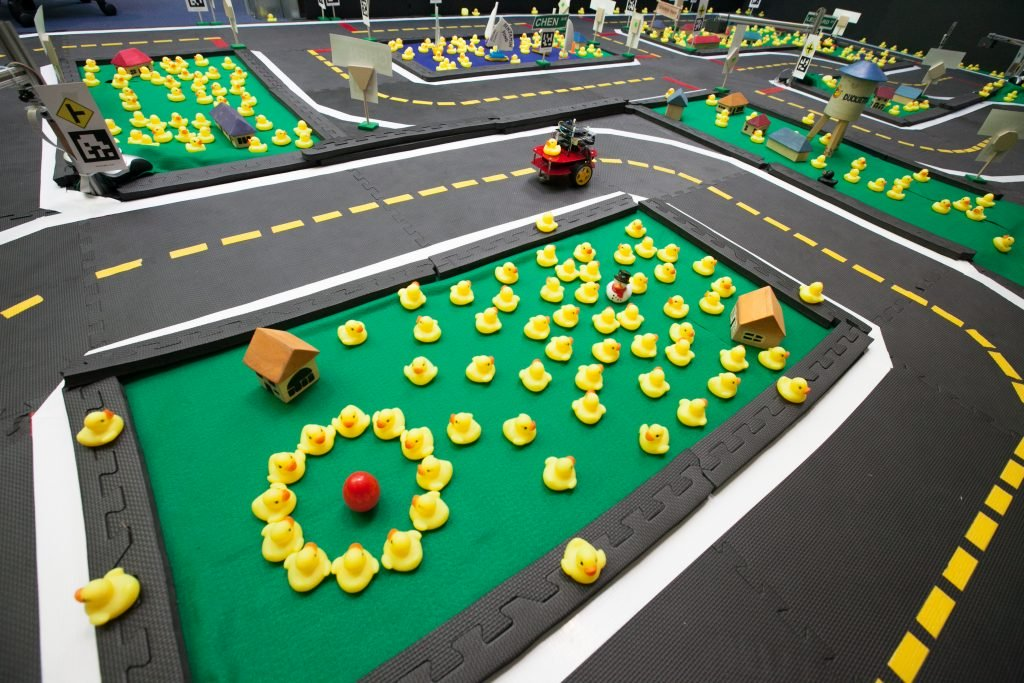
\includegraphics[width=0.95\textwidth]{kapitel1/images/duckietown.png}
		\quelle\url{https://www.duckietown.org/wp-content/uploads/2018/05/duckietown_nice-1024x683.jpg}
		\label{fig:duckietown}
	\end{minipage}%
	\begin{minipage}{.5\textwidth}
		\centering
		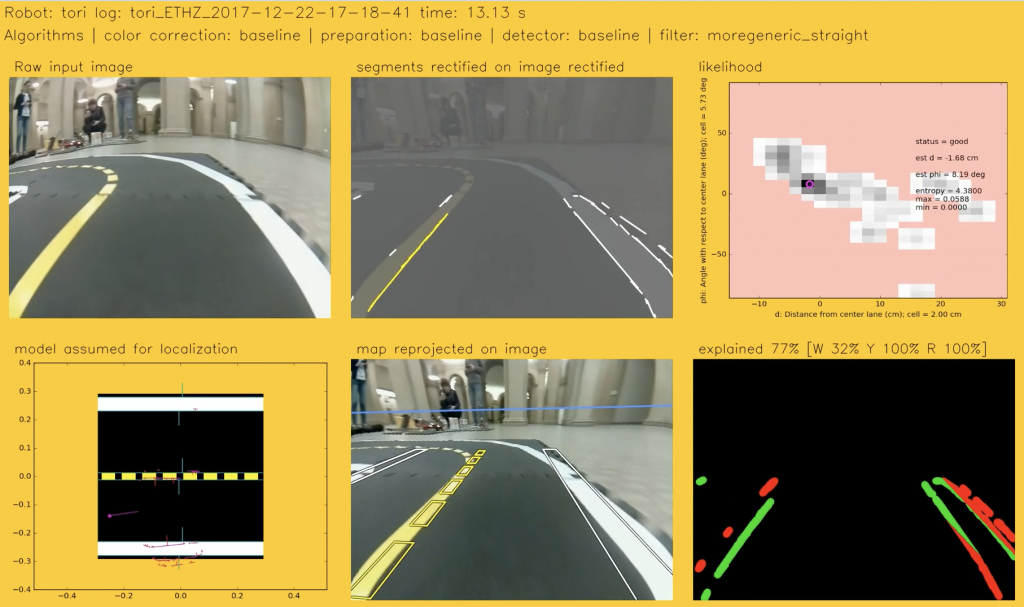
\includegraphics[width=1.072\textwidth]{kapitel1/images/duckietown2.png}
		\quelle\url{https://www.duckietown.org/wp-content/uploads/2018/06/data-from-img-CameraDataProcessed-fc6fd822-1024x607.png}
		\label{fig:duckietown2}
	\end{minipage}
	\caption{DuckieTown}
\end{figure}

Das DuckieTown-Projekt wurde 2016 am \acf{mit} konzipiert. Das Ziel war es, eine Plattform zu
entwickeln, die klein, kostengünstig und \grqq smart\grqq{} ist, aber dennoch die wissenschaftlichen
Herausforderungen einer echten autonomen Roboterplattform anbietet und die Entwicklung
intelligenter autonomer Fahrfunktionen erlaubt. \cite{duckietown}\\

\noindent Ziel des AIN-Projekts ist die Implementierung verschiedener klassischer Robotik-Algorithmen
für Navigation und Lokalisierung mit dem DuckieTown-Simulator\\

\noindent Nach einer Einarbeitung in die Fähigkeiten des Simulators sollen Algorithmen für die
Linienverfolgung, Lokalisierung mit einem Partikelfilter bei bekannter Umgebungskarte,
Navigation (Planung, Wegeverfolgung und Hindernisvermeidung) realisiert werden. Optional können auch KI-Komponenten für
Fahrverhalten und Erkennung von Verkehrszeichen entwickelt werden. Hierzu sollen neue
Techniken wie Deep Neural Networks und Deep Reinforcement Learning zum Einsatz
kommen.\\

\noindent Das Projekt, das für etwa 4-6 Personen in zwei bis drei Teams vorgesehen ist, soll in Python realisiert werden.
Eventuell kommt das \acf{ros} zum Einsatz.

\newpage

\section{Aufgabenstellung}

Das Ziel unseres Teams ist die Auswertung der Kamerabilder eines Agenten in einer DuckieTown-Umgebung. Mit den daraus gewonnenen Informationen soll der Agent in der Lage sein, vollständig autonom die Fahrspur halten zu können. Benötigt wird daher ein System, welches anhand einer Kameraaufnahme Steuerbefehle für den Agenten berechnet.

Ein weiteres mögliches Ziel ist die Nutzung der Informationen zur Lokalisierung des Agenten. Über Odometrie kann die Orientierung relativ zur Startpose geschätzt werden. Weißt die Trajektorie über einen gewissen Zeitraum eine Änderung der Orientierung von etwa 90 \acs{bzw} 270 Grad auf, kann davon ausgegangen werden, dass der Agent eine Kurve durchfahren hat. Ist außerdem die Umgebungskarte bekannt, kann mit Hilfe eines Monte-Carlo-Verfahrens der Agent global lokalisiert werden.\\

Wir werden zur Berechnung des Steuerbefehls auf zwei Ansätze eingehen:

\begin{itemize}
	\item Inferenz der Pose des Agenten:\\
	Aus der Aufnahme wird zunächst die relative Pose des Agenten zur Fahrspur inferiert. Diese besteht aus dem kürzesten Abstand $d$ zu einer Straßenmarkierung, sowie aus der Winkeldifferenz $\theta$ zwischen Orientierung des Agenten und der Fahrbahn. Diese Werte werden dann mit einem \acs{pid}-Regler konstant gehalten.\\
	Dieser Ansatz hat den Vorteil, dass die Poseninformationen außerdem noch für die schnellere Lokalisierung des Agenten genutzt werden können, da das Durchfahren einer Kurve von dem Fahren von Schlangenlinien unterschieden werden kann, wenn die Steuerbefehle mit $d$ abgeglichen werden.
	\item Direkte Inferenz des Steuerbefehls:\\
	Der weiter verbreitete Ansatz der direkten Inferenz übergeht die Schätzung der Pose. Anhand der Daten wird direkt ein Steuerbefehl geschätzt, bestehend aus der Geschwindigkeit $v$ und Winkelgeschwindigkeit $\omega$. Da für einen optimalen Steuerbefehl mehr Informationen nützlich sind als $d$ und $\theta$, ist dieser Ansatz ebenfalls vielversprechend. So kann ein Expertensystem für Steuerbefehle beispielsweise den weiteren Verlauf der Spur berücksichtigen, konkret die Winkeldifferenz zwischen der aktuellen Orientierung des Agenten und der Orientierung der Fahrspur an einem kommenden Zielpunkt.
\end{itemize}
